\subsubsection{Automatic}

One of our ultimate goal of the project is to use existing software and have a file-print process in which the MRI data is generated directly into a holographic print without any human intervention.  This automatic approach from MRI to holographic print needs automatic annotation and segmentation of the MRI data.  Current methods include the annotation and segmentation of each of the slices. This is inefficient and also time consuming. In this section we will explore the possibility of automating this step using transfer leaning and 3D U-Net dense volumetric segmentation\cite{cciccek20163d}.\\

One of the main issues using deep learning methods in the medical field, is the lack of a large enough sample size for the network to fully stabilize the weights and biases.  To overcome this issue it is often the case that we have to use transfer learning techniques using pre-trained networks.  In this project we explored the possibility of using inductive transfer learning\cite{pan2010survey} and a pre-trained network found in the work of \cite{cciccek20163d}.  Using transfer learning, instead of starting the learning process from the beginning, the learning process starts from patterns that have been learned when solving a different or similar problem. In this way, we essentially utilize previous learning's from the pre-trained network and apply them to our dataset.\\

The work done by \cite{cciccek20163d} expands the work previously achieved by \cite{ronneberger2015u} but using 3D volumetric data.  There is an added dimension of depth in all filters and weights in the U-Net architecture.  The depth information comes from the slice information in the MRI. During the encoder or down sampling portion of the architecture two 3 x 3 x 3 convolutions were performed followed by a rectified linear unit (ReLu).  This was followed up by a single 2 x 2 x 2 max pooling with strides of 2 in each dimension.  In the synthesis or up-convolution path a 2 x 2 x 2 with strides of 2 in each dimension was used followed by the mirrored 3 x 3 x 3 convolution with ReLu.  To reduce bottle-necking doubling the channels was done before each max pooling layer.  In the last layer a 1 x 1 x 1 x 1 convolution was used for the output layer for each of the labeled cases white matter, gray matter, tumor and abnormal tissue. The last layer used a weighted softmax loss function.  Note that the input layer was 256 x 256 x 118.

\begin{figure}[H]
  \centering
  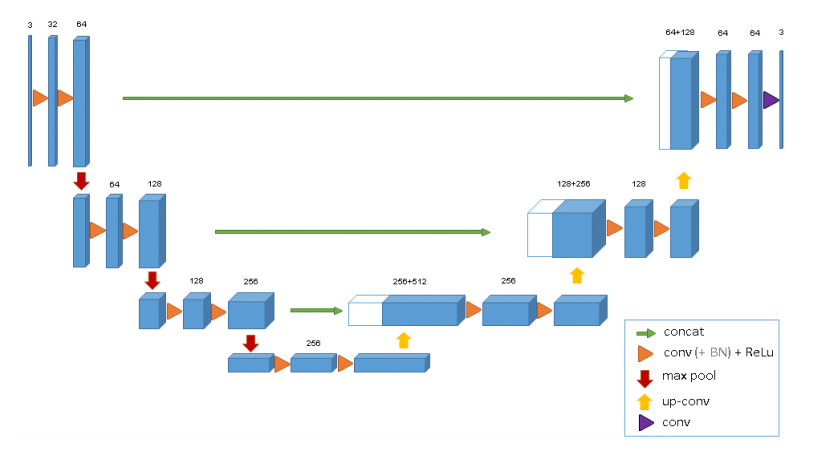
\includegraphics[width=\linewidth]{img/volumetricUNetArchitecture.PNG}
  \caption{UNet architecture used in Cicek et.el. \cite{cciccek20163d}}
  \label{fig:uNet}
\end{figure}

In theory this approach would have worked but the data used by \cite{cciccek20163d} was too different from the data we are using, so the transfer learning did not give us the adequate segmentation we wanted.  Due to the limited time of the project this was abandoned and semi-automatic techniques were more focused as they are more intuitive and don't require a large sample size.  In the future we would like to pursue this approach as this would be more akin to our ultimate goal of the file-print process.
